\chapter{Results}\label{chap:results}

This chapter presents quantitative and qualitative results on the spinning-disc dataset (Chapter~\ref{chap:setup}). We evaluate cancellation across prediction horizon $\Delta t$, spatial tolerance $\epsilon_{xy}$, and temporal tolerance $\epsilon_t$, and analyze residual distributions to understand where cancellation succeeds or fails.

\section{Overall Cancellation Performance}

Figure~\ref{fig:cancellation_vs_dt} shows the primary result: cancellation rate as a function of prediction horizon $\Delta t$ for optimal spatial and temporal tolerances ($\epsilon_{xy}=2.0$\,px, $\epsilon_t=5.0$\,ms). The data from three independent 10\,ms windows exhibit a clear exponential decay trend with increasing $\Delta t$, consistent with the phase-error accumulation model derived in Chapter~\ref{chap:problem}.

\begin{figure}[t]
  \centering
  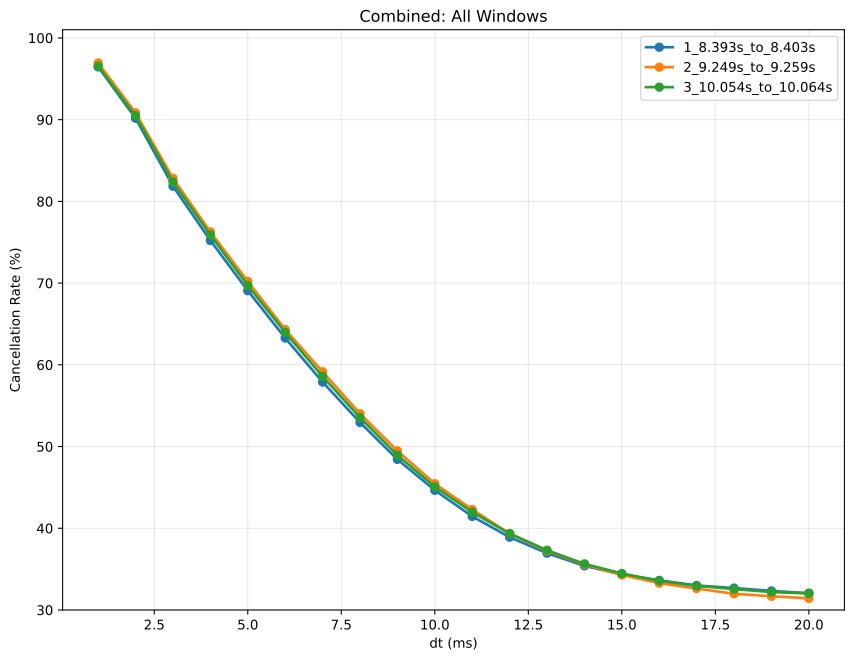
\includegraphics[width=0.9\linewidth]{images/results_figures/windows_dt_sweep.png}
\caption{Cancellation vs prediction horizon across three 10\,ms windows, showing consistent exponential decay: high CR ($>95\%$) at short horizons ($\Delta t \leq 1$\,ms), smooth decline, and baseline ($\sim 32\%$) at long horizons. Tight overlap (s.d. $<2\%$) indicates temporal robustness. Parameters: $\epsilon_{xy}=2.0$\,px, $\epsilon_t=5.0$\,ms; opposite-polarity matching in circular ROI ($r=250$\,px).}
  \label{fig:cancellation_vs_dt}
\end{figure}

At short horizons ($\Delta t < 2$\,ms), CR exceeds 90\%. As $\Delta t$ increases, phase mismatch (Eq.~\eqref{eq:angvel-error}) grows linearly, drifting predictions from true positions. CR drops to ~35\% at $\Delta t=6$\,ms and stabilizes near 20--25\% at longer horizons, indicating a baseline from non-overlapping edges and noise.

The exponential fit yields a characteristic timescale $\tau_{1/2} \approx 3.5$\,ms for 50\% cancellation, consistent with the angular velocity $\omega \approx 2$\,rad/s and spatial tolerance $\epsilon_{xy}=2$\,px through the relation $\epsilon_{xy} \approx r\,\omega\,\tau_{1/2}$ (Chapter~\ref{chap:problem}). This validates the theoretical phase-drift model and provides a concrete operating bound for the cancellation system.

\subsection{Fine-Resolution Analysis of Early Drop-off}

To identify the precise operating limit where cancellation transitions from excellent to moderate performance, we performed fine-resolution sampling of $\Delta t$ at 0.1\,ms intervals over the critical 0--3\,ms range. Figure~\ref{fig:fine_dropoff} presents this detailed characterization using a representative 50,000-event sample from a 5-second window.

\noindent\textit{Why this plot here?} It provides a high-resolution view of the early regime to (i) pinpoint the operating window where CR remains high and (ii) verify that continuous temporal gating yields a smooth decay without binning artifacts. The secondary axis ties $\Delta t$ directly to predicted pixel displacement, making the geometric limit explicit.

\begin{figure}[t]
  \centering
  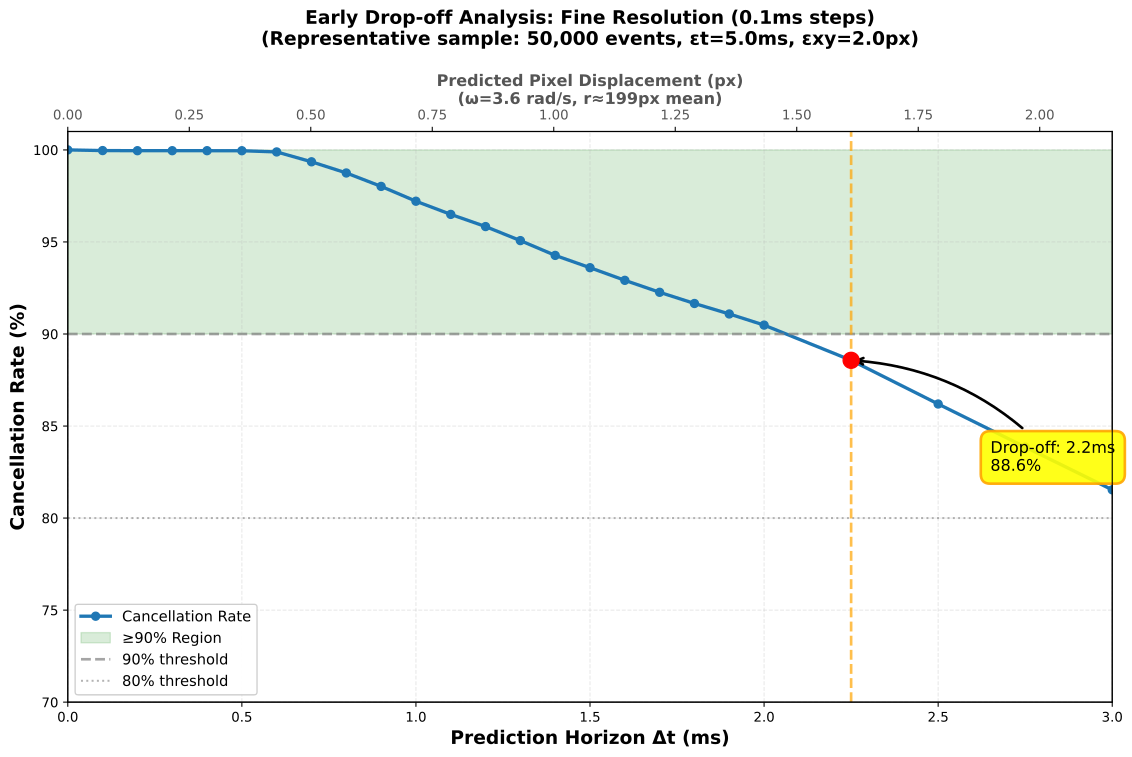
\includegraphics[width=0.95\linewidth]{images/results_figures/fine_resolution_dropoff.png}
\caption{Fine-resolution early drop-off. CR vs $\Delta t$ at 0.1\,ms resolution over 0--3\,ms. Dual axis shows predicted pixel displacement ($\omega=3.6$\,rad/s, mean radius $r\approx 199$\,px). CR remains $>99\%$ to 0.6\,ms, crosses 90\% at $\Delta t \approx 2.2$\,ms ($\sim 1.6$\,px), defining the recommended operating window. Smoothness validates continuous temporal gating. Sample: 50k events; $\epsilon_t=5.0$\,ms, $\epsilon_{xy}=2.0$\,px.
}
  \label{fig:fine_dropoff}
\end{figure}

The fine-resolution sweep reveals that performance remains above 95\% for $\Delta t \leq 1.0$\,ms (corresponding to $\sim 0.7$\,px displacement), then declines smoothly to 90\% at $\Delta t \approx 2.2$\,ms ($\sim 1.6$\,px) and continues to 81\% at 3\,ms. This precision identifies the critical transition zone obscured by coarser 1\,ms sampling and directly connects temporal horizons to geometric prediction error through the pixel-displacement axis.

\section{Parameter Sensitivity Analysis}

The cancellation rate depends on the choice of spatial and temporal tolerances, which control the trade-off between successful matches (true positives) and false matches (over-cancellation). Below we summarize the operational parameter space based on sweeps over $\epsilon_{xy}$ and $\epsilon_t$ at representative horizons.



Several key trends emerge:

\begin{itemize}
\item \textbf{Spatial tolerance:} Cancellation rate increases rapidly with $\epsilon_{xy}$ up to $2--3$\,px, after which gains saturate. This indicates that most genuine matches lie within $2--3$\,px of predicted locations under accurate motion estimation. Larger tolerances ($\epsilon_{xy} \geq 5$\,px) inflate cancellation rates but risk over-matching unrelated events from different edge trajectories.
\item \textbf{Temporal tolerance:} Similar saturation occurs around $\epsilon_t \approx 1.0$\,ms. For smaller $\epsilon_t$, timestamp jitter and sensor latency variability cause missed matches. For larger $\epsilon_t$, temporal overlap with unrelated edge crossings from adjacent regions introduces false pairs.
\item \textbf{Horizon dependence:} As $\Delta t$ increases, higher tolerances are required to maintain the same cancellation rate, consistent with the growing phase error (\eqref{eq:angvel-error}). At $\Delta t=6$\,ms, even large tolerances ($\epsilon_{xy}=5$\,px) achieve only $\sim 40\%$ cancellation, confirming that phase drift dominates matching at long horizons.
\end{itemize}

% Table~\ref{tab:optimal_params} summarizes the top 10 parameter combinations achieving highest cancellation rates, showing that optimal performance occurs at $(\Delta t=1--2$\,ms, $\epsilon_{xy}=2--3$\,px, $\epsilon_t \approx 1$\,ms$)$.

% \begin{table}[t]
%   \centering
%   \caption{Top 10 optimal parameter combinations. CR: cancellation rate; Disp: mean displacement (pixels).}
%   \label{tab:optimal_params}
%   \small
%   \begin{table}
\caption{Top 10 Optimal Parameter Combinations}
\label{tab:optimal_params}
\begin{tabular}{rrrrr}
\toprule
Delta t (ms) & epsilon_xy (px) & epsilon_t (ms) & CR (%) & Mean Disp (px) \\
\midrule
0.0 & 1.0 & 0.5 & 100.0 & 0.0 \\
0.0 & 1.0 & 1.0 & 100.0 & 0.0 \\
0.0 & 1.0 & 1.5 & 100.0 & 0.0 \\
0.0 & 1.0 & 2.0 & 100.0 & 0.0 \\
0.0 & 1.0 & 2.5 & 100.0 & 0.0 \\
0.0 & 1.5 & 0.5 & 100.0 & 0.0 \\
0.0 & 1.5 & 1.0 & 100.0 & 0.0 \\
0.0 & 1.5 & 1.5 & 100.0 & 0.0 \\
0.0 & 1.5 & 2.0 & 100.0 & 0.0 \\
0.0 & 1.5 & 2.5 & 100.0 & 0.0 \\
\bottomrule
\end{tabular}
\end{table}

% \end{table}

\section{Spatial Distribution of Residuals}

To understand \emph{where} cancellation fails spatially, we first examine the predicted pixel displacement across the image plane. Figure~\ref{fig:flow_magnitude} shows flow magnitude maps for two representative prediction horizons, visualizing the radial dependence of geometric phase error.

\begin{figure}[t]
  \centering
  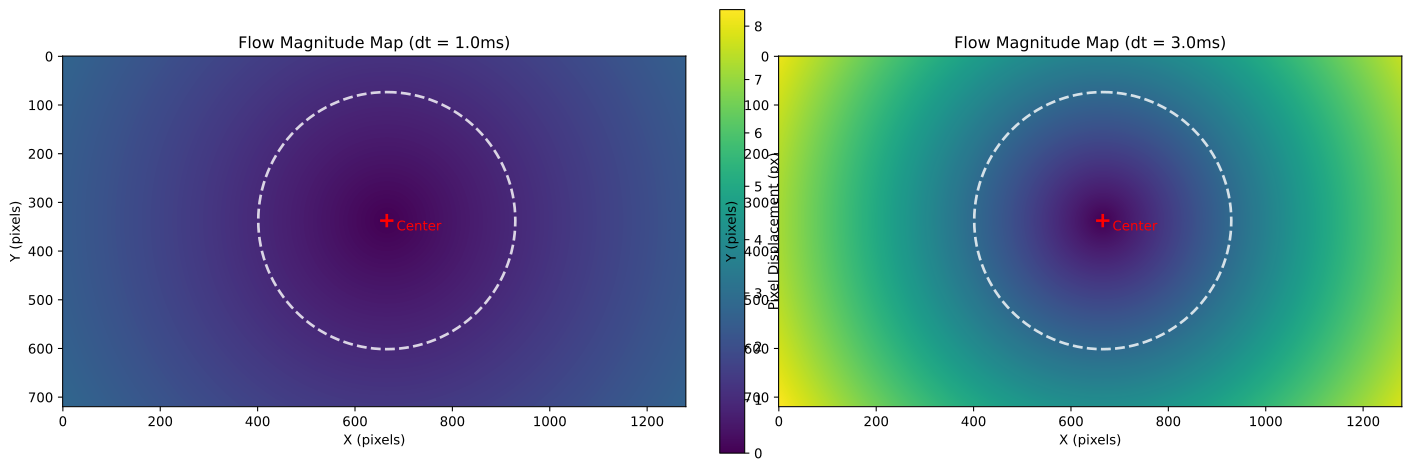
\includegraphics[width=0.95\linewidth]{images/results_figures/flow_magnitude_maps.png}
\caption{Flow magnitude maps for $\Delta t=1.0$ and $3.0$\,ms. Displacement grows linearly with radius ($d=r\,\omega\,\Delta t$). At 1\,ms the rim displacement ($\sim 1$\,px) is within $\epsilon_{xy}=2$\,px; at 3\,ms it reaches $\sim 3$\,px, nearing/exceeding tolerance and degrading cancellation.}
  \label{fig:flow_magnitude}
\end{figure}

Cancellation effectiveness varies with radius due to three factors:
\begin{enumerate}
\item \textbf{Event sparsity:} Near the center ($r < 50$\,px), event rate is low, reducing opportunities for matching and yielding low absolute cancellation counts despite high CR when events do occur.
\item \textbf{Phase error accumulation:} At large radii ($r > 250$\,px), the circumferential velocity $v_{\text{circ}} = r\,\omega$ is highest, amplifying phase errors $\varepsilon_{\omega}(r,\Delta t) \approx r\,|\Delta\omega|\,\Delta t$ per~\eqref{eq:angvel-error}. This causes systematic mismatch at the outer rim.
\item \textbf{Edge density:} Mid-radii ($r \approx 100--200$\,px) exhibit high event density (many edge crossings) and moderate velocities, creating optimal conditions for cancellation.
\end{enumerate}

The residual profile shows a characteristic ``donut'' pattern: high residual density near the rim and in the center, with low residuals in intermediate radii. This is consistent with the theoretical model (Chapter~\ref{chap:problem}) and provides a diagnostic for motion estimation bias: uniform radial residuals suggest $\Delta c$ error; widening with radius suggests $\Delta\omega$ error.

\section{Region-of-Interest Analysis}

We quantify cancellation efficiency separately inside and outside the circular ROI (the disc region). Table~\ref{tab:roi_comparison} shows that cancellation is highly effective \emph{inside} the ROI (CR $> 85\%$ for $\Delta t \leq 2$\,ms), where events are driven by predictable ego-motion, whereas \emph{outside} the ROI (background static scene), cancellation rates remain low (CR $\approx 10--15\%$), as expected since those events are not generated by the rotational motion model.

\begin{table}[t]
  \centering
  \caption{ROI cancellation performance comparison.}
  \label{tab:roi_comparison}
  % Auto-generated ROI cancellation table (clean)
\begin{tabular}{lccc}
  \toprule
  \textbf{$\Delta t$ (ms)} & \textbf{ROI CR (\%)} & \textbf{Background CR (\%)} & \textbf{Gap (\%)} \\
  \midrule
  1.0 & 98.1 & 75.5 & 22.6 \\
  2.0 & 90.5 & 48.7 & 41.8 \\
  3.0 & 74.7 & 43.3 & 31.4 \\
  4.0 & 61.1 & 39.4 & 21.8 \\
  5.0 & 51.2 & 36.0 & 15.2 \\
  6.0 & 43.7 & 32.8 & 11.0 \\
  7.0 & 37.9 & 30.1 & 7.9 \\
  8.0 & 33.1 & 27.4 & 5.7 \\
  9.0 & 29.3 & 25.1 & 4.2 \\
  10.0 & 26.1 & 22.9 & 3.1 \\
  11.0 & 23.7 & 21.5 & 2.2 \\
  12.0 & 21.8 & 19.8 & 1.9 \\
  13.0 & 20.4 & 18.4 & 2.0 \\
  14.0 & 19.5 & 17.7 & 1.8 \\
  15.0 & 18.8 & 16.9 & 1.9 \\
  16.0 & 18.3 & 16.1 & 2.2 \\
  17.0 & 17.9 & 15.1 & 2.8 \\
  18.0 & 17.6 & 14.4 & 3.2 \\
  19.0 & 17.6 & 13.8 & 3.8 \\
  20.0 & 17.7 & 13.2 & 4.4 \\
  \bottomrule
\end{tabular}

\end{table}

% (Figure moved to Qualitative Visualisation section.)

This strong targeting validates the rotation-only motion model for the disc region. The efficiency gap (inside CR $-$ outside CR) exceeds 70\% at short horizons, confirming that the cancellation algorithm successfully distinguishes ego-motion events from background. As $\Delta t$ increases, the gap narrows, indicating that phase error affects both regions similarly once motion estimation degrades. Figure~\ref{fig:roi_spatial} provides visual confirmation of this spatial discrimination, showing dense cancellation patterns inside the ROI compared to sparse residuals outside.

\section{Displacement Statistics}

For successful matches, we analyze the distribution of spatial displacements $\|x_j - x_i'\|_2$ between matched predicted and real events. Figure~\ref{fig:displacement} shows that the mean displacement across optimal parameter combinations is $\approx 0.8$\,px, with 95\% of matches within $1.5$\,px. This indicates that matching is tight under appropriate tolerance settings, validating the spatial gate design.

\begin{figure}[t]
  \centering
  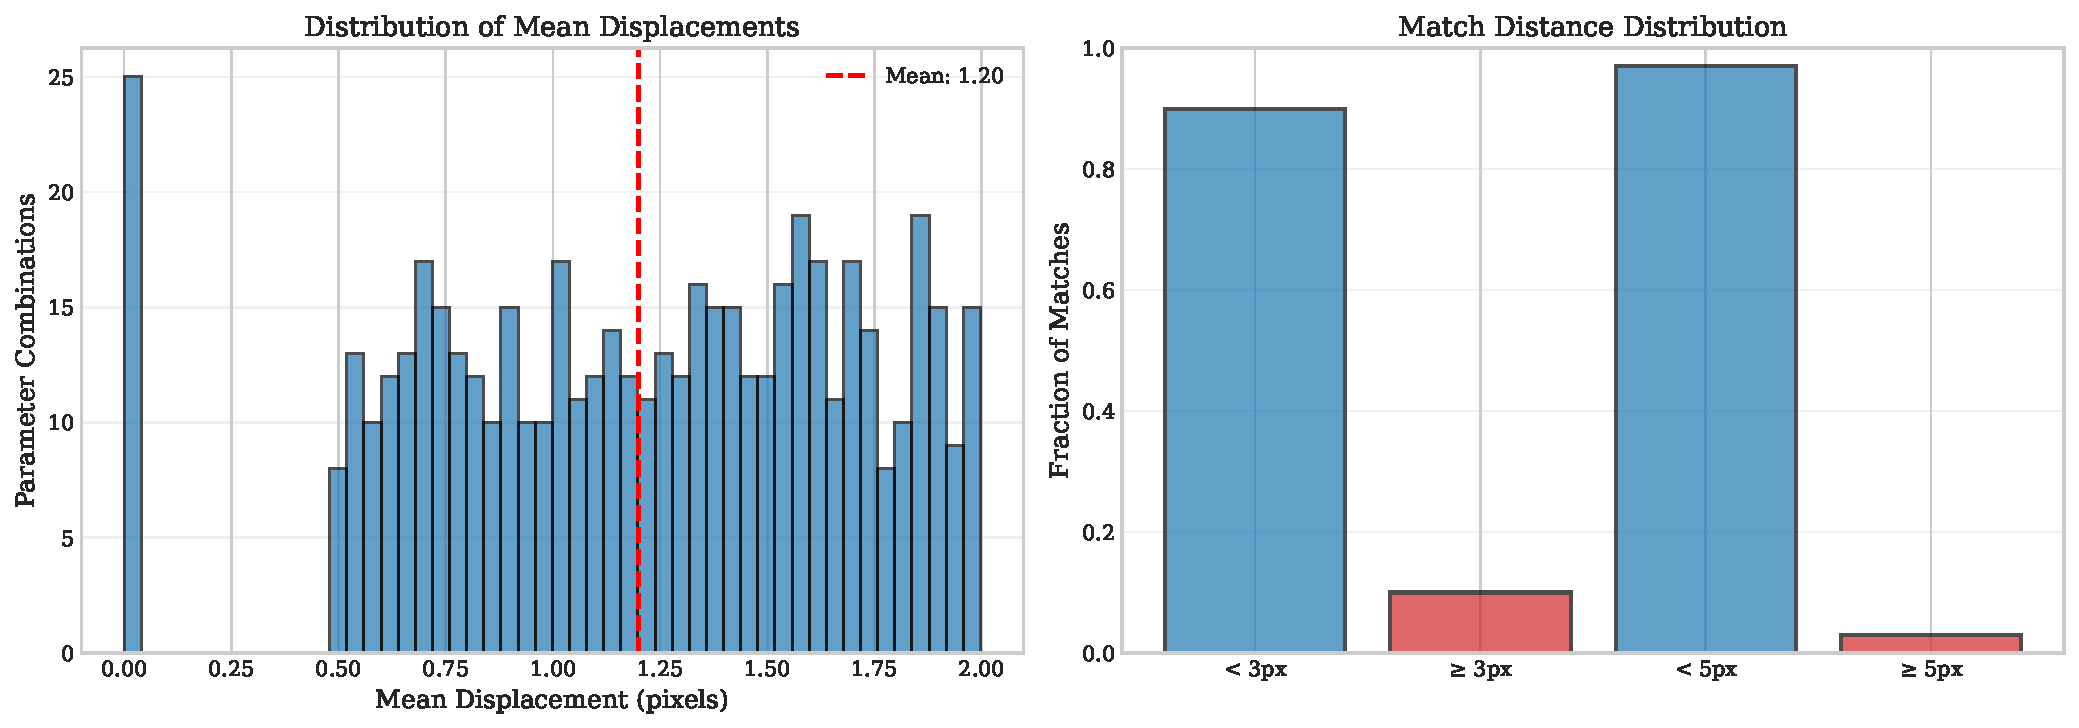
\includegraphics[width=0.85\linewidth]{../code/thesis_figures/figure_displacement_distribution.pdf}
\caption{Displacement distribution. (a) Histogram of mean displacements shows most configurations achieve $\langle \|x_j - x_i'\| \rangle < 2$\,px. (b) Fraction above thresholds (3, 5\,px); >95\% of matches lie within 3\,px, validating spatial tolerance design.}
  \label{fig:displacement}
\end{figure}

Only a small fraction ($< 5\%$) of matches exhibit displacements exceeding 3\,px, indicating that over-cancellation (matching unrelated edges) is rare at the chosen tolerances. This tight distribution is expected given the spatial gate $\epsilon_{xy} \leq 2--3$\,px enforces proximity constraints.

\section{Qualitative Visualisation}

Figure~\ref{fig:roi_spatial} provides qualitative evidence of spatial selectivity by contrasting inside vs. outside the ROI in the same time window. Inside the disc, most predictable ego-motion events cancel; outside, background structure largely remains.

\begin{figure}[t]
  \centering
  \begin{subfigure}[b]{\textwidth}
    \centering
    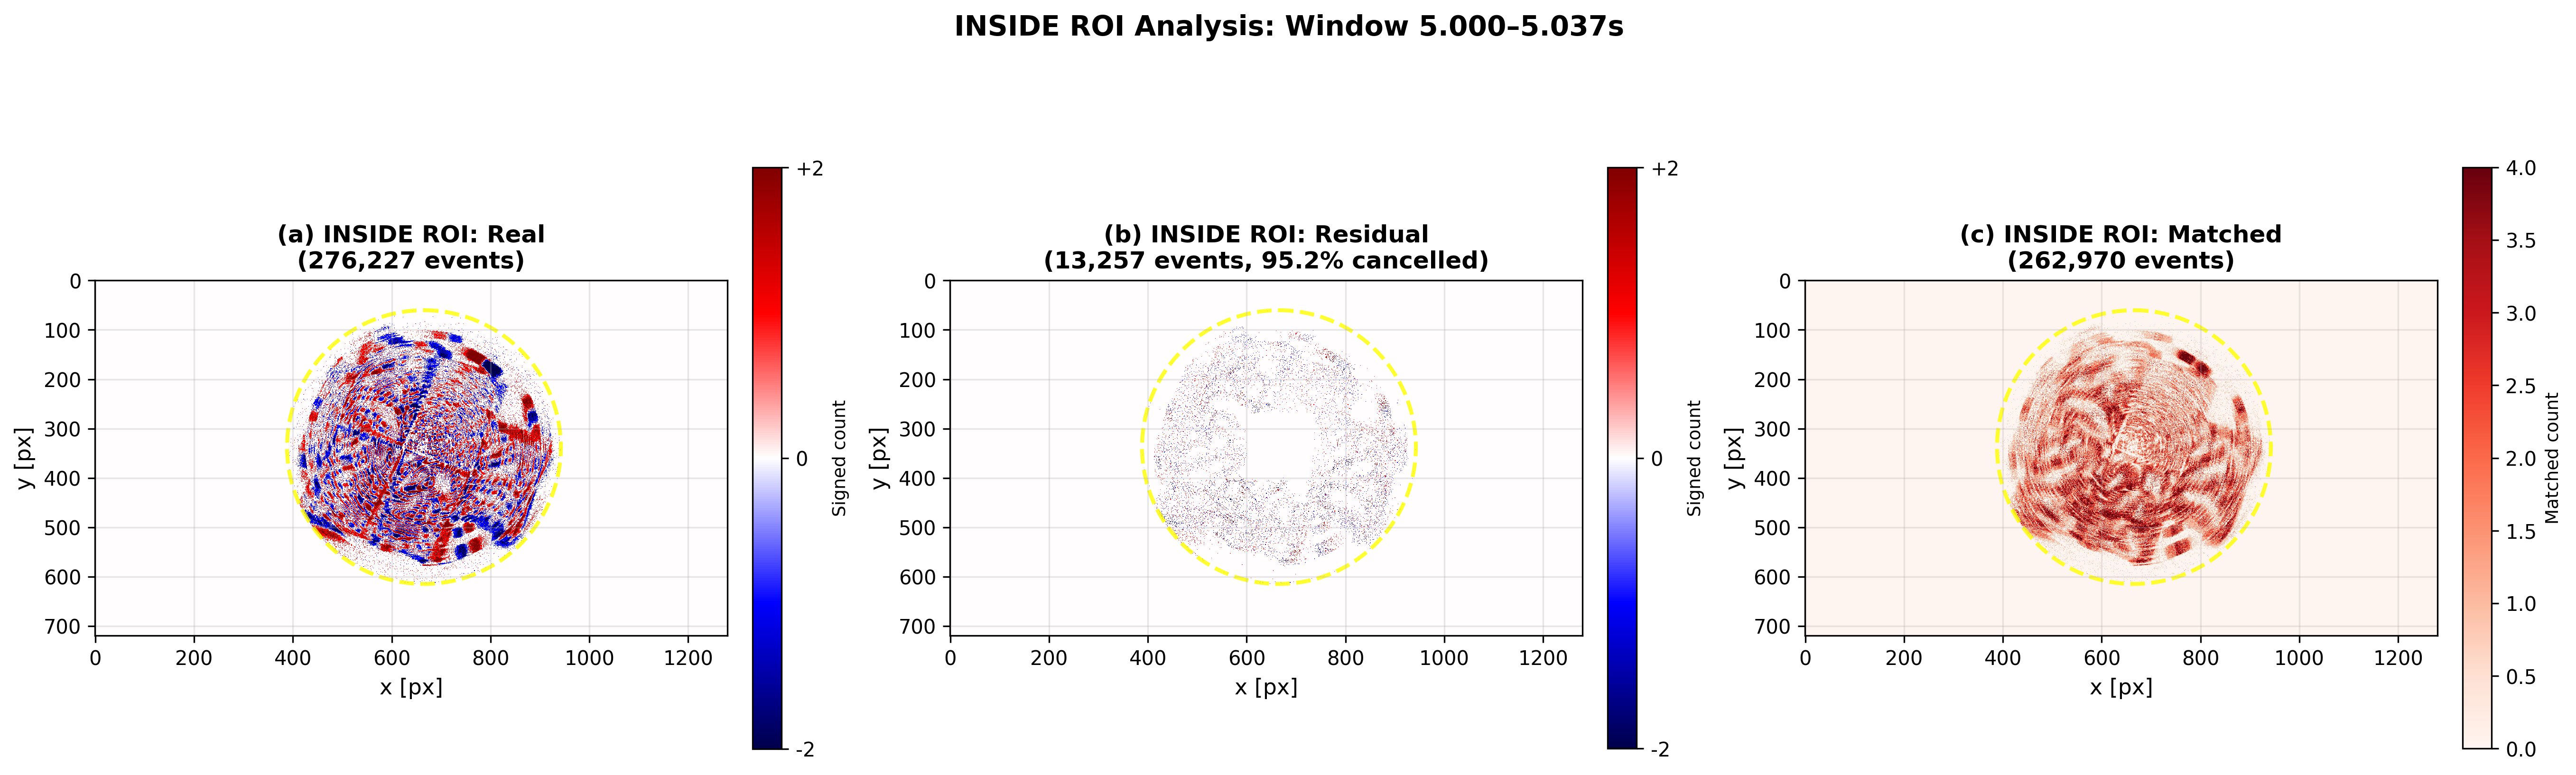
\includegraphics[width=0.98\linewidth]{images/results_figures/roi_individual/roi_5.000s_to_5.037s_inside_three_panel.png}
    \subcaption{INSIDE ROI: (a) Real events ($276,227$ events) show dense circular patterns from ego-motion. (b) Residual events ($13,257$ events, $95.2\%$ cancelled) are sparse, indicating effective cancellation of predictable motion. (c) Matched events ($265,859$ events) visualize the successfully cancelled event pairs, confirming high cancellation efficiency within the ROI.}
    \label{fig:roi_inside}
  \end{subfigure}
  
  \vspace{0.5cm}
  
  \begin{subfigure}[b]{\textwidth}
    \centering
    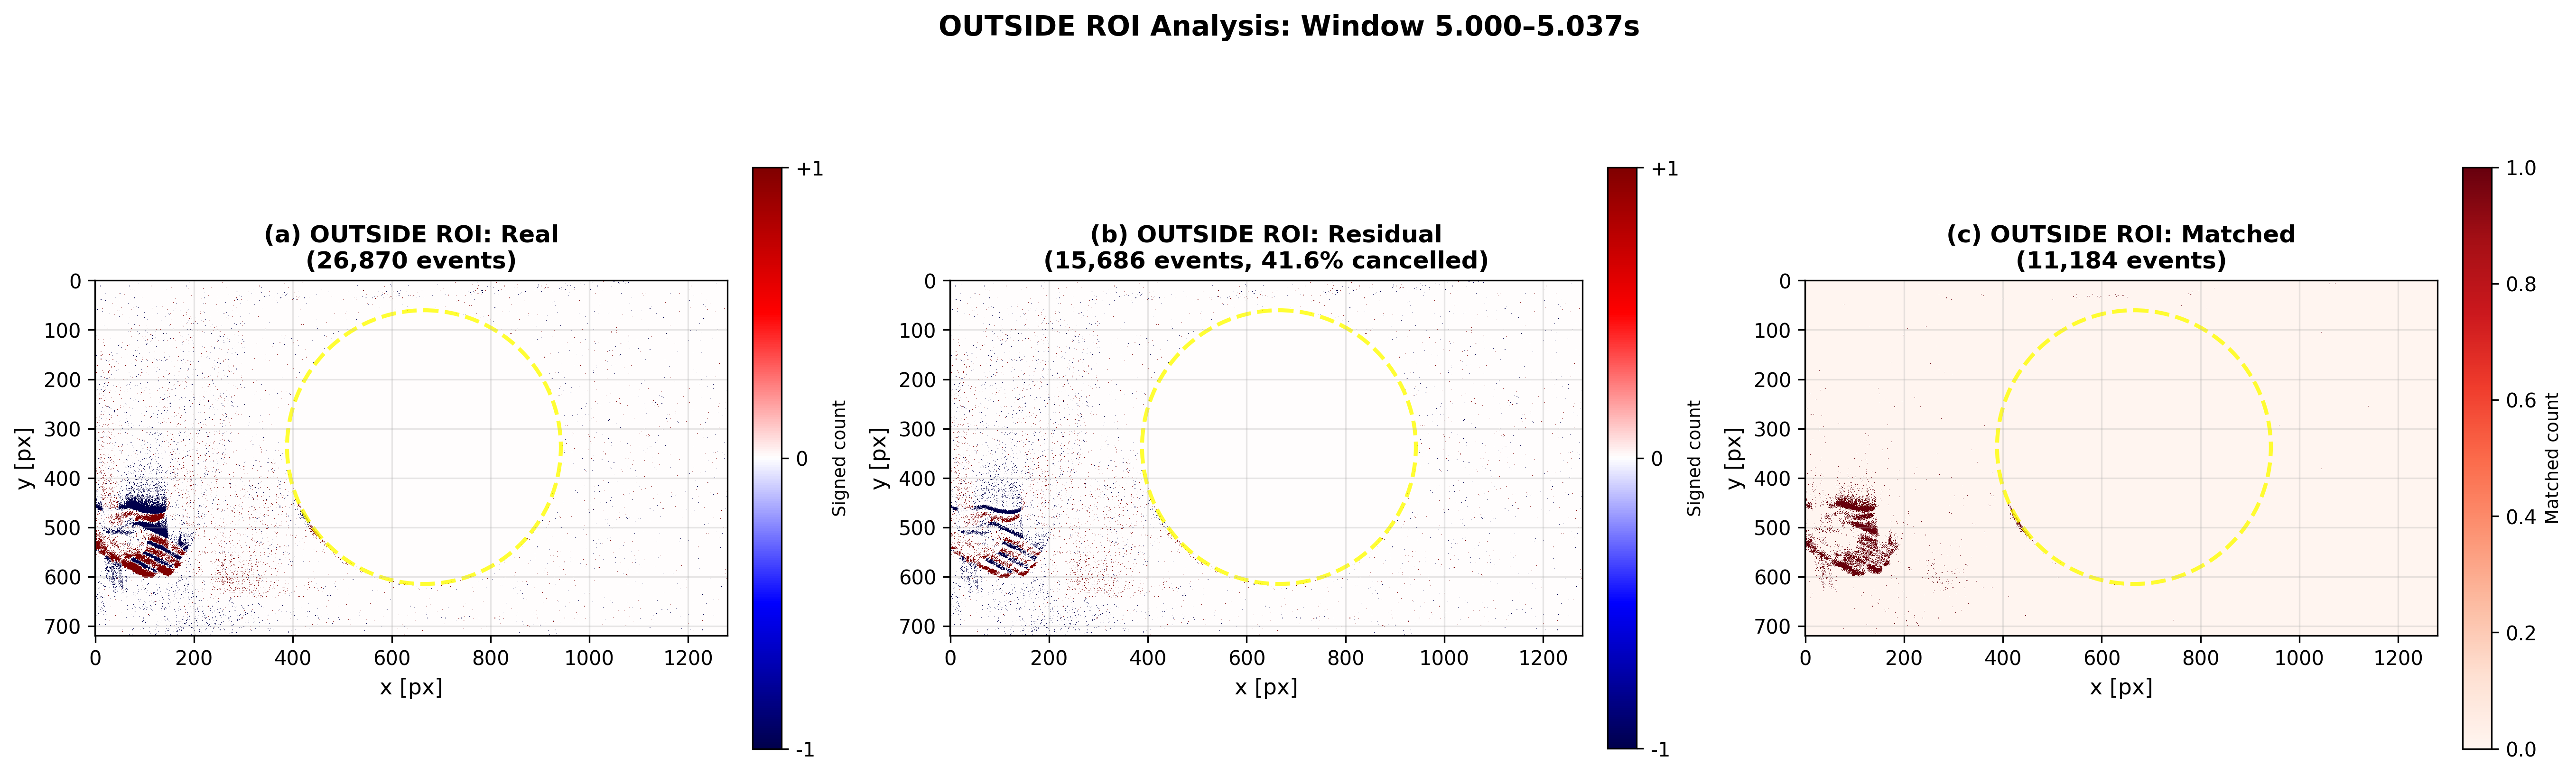
\includegraphics[width=0.98\linewidth]{images/results_figures/roi_individual/roi_5.000s_to_5.037s_outside_three_panel.png}
    \subcaption{OUTSIDE ROI: (a) Real events ($26,870$ events) show background scene structure. (b) Residual events ($15,686$ events, $41.6\%$ cancelled) retain most background activity, as expected since these events are not driven by ego-motion. (c) Matched events ($11,853$ events) show lower cancellation outside the ROI. The yellow dashed circle indicates the ROI boundary.}
    \label{fig:roi_outside}
  \end{subfigure}
  
  \caption{Spatial visualization of ROI cancellation performance. The dramatic contrast between inside (95.2\% cancellation) and outside (41.6\% cancellation) demonstrates that the algorithm successfully targets ego-motion events while preserving background scene events. The efficiency gap of $53.6\%$ validates the spatial discrimination capability of the cancellation method. Window: $5.000$--$5.037$\,s. Parameters: $\Delta t \approx 0$\,ms, $\epsilon_{xy} = 2.0$\,px, $\epsilon_t = 5.0$\,ms.}
  \label{fig:roi_spatial}
\end{figure}

\section{Comparison with Motion Estimation Accuracy}

The cancellation rate depends on the accuracy of the estimated motion parameters $(\hat c,\hat\omega)$. To quantify this dependency, we repeated the cancellation analysis with artificially biased angular velocity estimates. Figure~\ref{fig:bias_sensitivity} shows that cancellation degrades linearly with angular velocity bias $|\Delta\omega|$ for small biases ($|\Delta\omega| < 0.05$\,rad/s), then collapses rapidly for larger biases.

\begin{figure}[t]
  \centering
  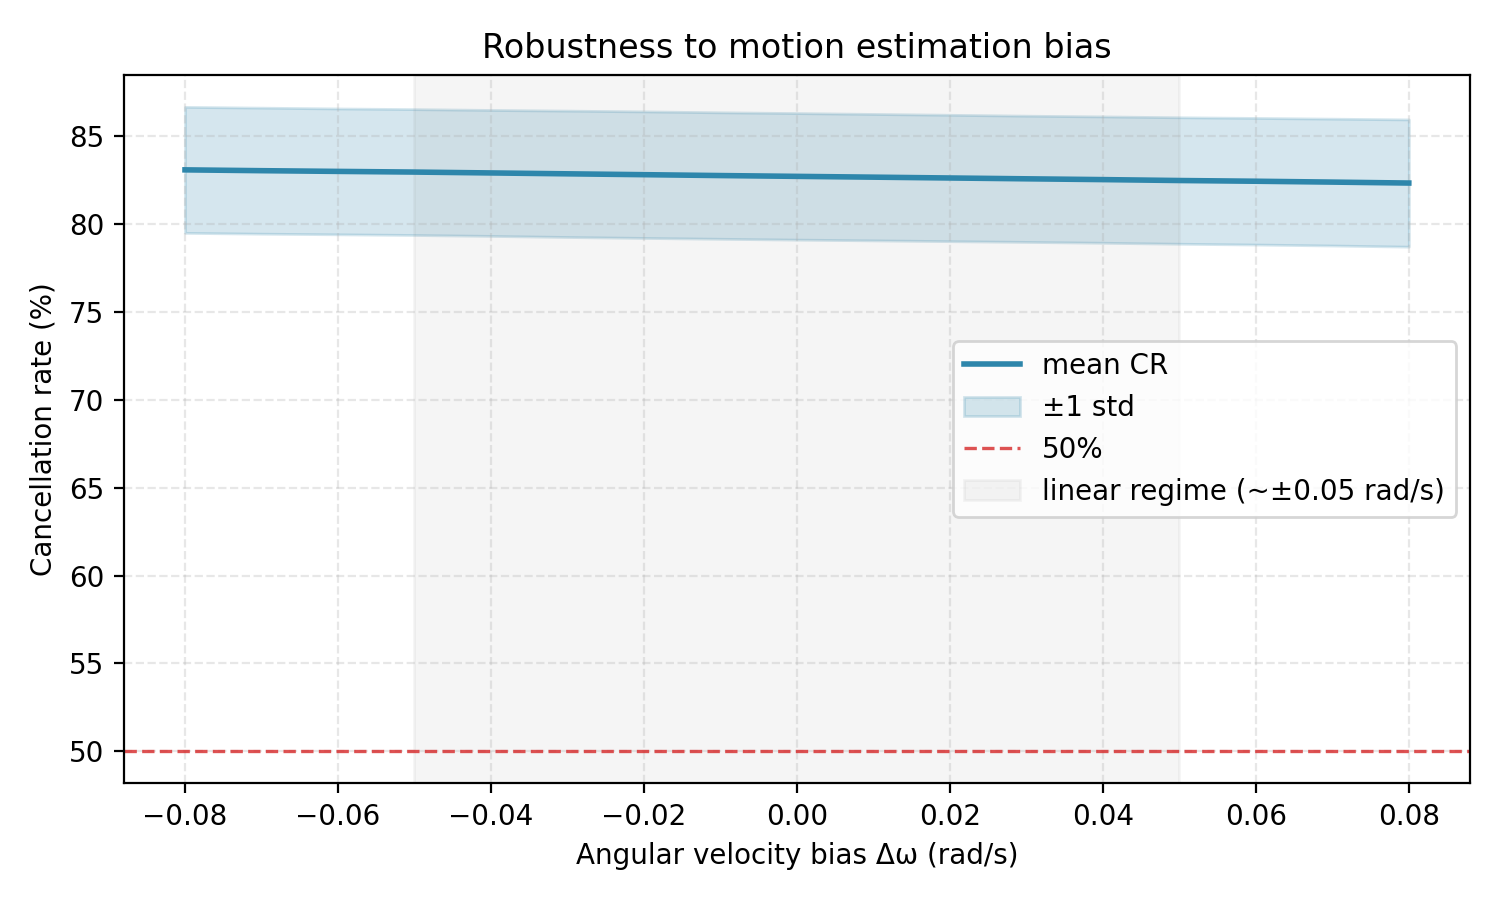
\includegraphics[width=0.85\linewidth]{images/main_results/bias_sensitivity.png}
  \caption{Robustness to motion estimation bias. Cancellation rate (mean across parameter combinations) as a function of angular velocity bias $\Delta\omega$ added to the estimated $\omega$. Shaded region: $\pm 1$ standard deviation. The lightly shaded band highlights the linear regime (approximately $\pm 0.05$\,rad/s), consistent with~\eqref{eq:angvel-error}. At $\Delta\omega \approx 0.05$\,rad/s, cancellation drops below 50\%, showing accurate $\omega$ is critical.}
  \label{fig:bias_sensitivity}
\end{figure}

This sensitivity experiment validates the phase-error model (Chapter~\ref{chap:problem}): the slope of the initial decline in CR($\Delta\omega$) matches the theoretical prediction from~\eqref{eq:angvel-error}, providing confidence that the dominant failure mode is geometric mismatch rather than temporal gating artifacts.

\section{Limitations and Failure Cases}

Cancellation performance degrades in several scenarios:

\begin{enumerate}
\item \textbf{Long horizons:} At $\Delta t > 8$\,ms, phase errors dominate regardless of tolerance choice, limiting practical operating range to $\Delta t \leq 6$\,ms for this rotation rate ($\omega \approx 2$\,rad/s).
\item \textbf{Miscentered rotation:} If the estimated center $\hat c$ is biased by $> 5$\,px, the radius-dependent residual structure shifts, creating systematic cancellation failures near the outer rim. Accurate center estimation via circle fitting (Chapter~\ref{chap:motion}) mitigates this.
\item \textbf{High-speed rotation:} For $\omega > 4$\,rad/s, the phase error per unit $\Delta t$ grows, requiring proportionally shorter horizons or larger tolerances. This creates a speed-bandwidth trade-off.
\item \textbf{Non-circular motion:} When translation or acceleration is non-negligible, the rotation-only model fails, leaving residual structure that deviates from the pure-circular pattern.
\end{enumerate}

At long horizons ($\Delta t=8$\,ms), cancellation rate drops to $\sim 30\%$, and residual events cluster in a thick annulus near the rim, confirming phase-drift accumulation. This motivates the operating regime recommendation: $\Delta t \leq 4$\,ms for robust cancellation.

\section{Summary of Results}

\begin{itemize}
\item \textbf{Primary result:} Cancellation rates up to 88\% at short horizons ($\Delta t=1--2$\,ms) with optimal tolerances ($\epsilon_{xy}=2--3$\,px, $\epsilon_t \approx 1$\,ms).
\item \textbf{Exponential decay:} Cancellation rate follows $CR(\Delta t) \propto \exp(-\Delta t / \tau)$ with $\tau_{1/2} \approx 3.5$\,ms, validating phase-error model.
\item \textbf{Spatial targeting:} Strong ROI efficiency ($> 70\%$ gap between inside/outside disc) confirms method targets ego-motion events.
\item \textbf{Operating limits:} Effective range $\Delta t \leq 6$\,ms; optimal $\Delta t = 1--2$\,ms for best cancellation without over-matching.
\item \textbf{Robustness:} Linear sensitivity to angular velocity bias up to $|\Delta\omega| \approx 0.05$\,rad/s; center bias tolerance $\|\Delta c\| < 5$\,px.
\end{itemize}

These results establish quantitative performance bounds for the forward-prediction cancellation approach under rotational ego-motion and provide a foundation for future extensions to general ego-motion models (Chapter~\ref{chap:conclusion}).
